%%MaD.tex - Notes taken for Materials and Devices Lecture
%%Author: Andy Goetz
%%Date Modified: 10-7-09
%%License: Ask me before reproducing/modifying, etc.


\documentclass{article}

%Make sure you have the file ShumanNote.scy in the same directory as
%this one. It has contains the style sheet for ECE111, and is needed
%to standardize the layout of LateX documents created for the class.
\usepackage{ShumanNotes} 
\usepackage{tikz}
\usepackage{program}
\usepackage{listings}
\pdfpagewidth 8.5in 
\pdfpageheight 11in

%This package is used to line up pictures 
\usepackage{graphicx}
\usepackage{fancyvrb}
\usepackage{listings}
%allows cursive font
%\usepackage{amsmath}

%allows hyperlinks 
%\usepackage{hyperref}

\newcommand{\HRule}{\rule{\linewidth}{0.5mm}} 

\lhead{Homework 5}

\begin{document}

%% These commands allow me to use cursive letter for things such as
%% length.  Note that on ubuntu linux, this required installation of
%% the package 'texlive-fonts-extra'. 
%% Taken from
%% http://www.latex-community.org/forum/viewtopic.php?f=5&t=1404&start=0
\newenvironment{frcseries}{\fontfamily{frc}\selectfont}{}
\newcommand{\textfrc}[1]{{\frcseries#1}}
\newcommand{\mathfrc}[1]{\text{\textfrc{#1}}}

\section{Overview}
Below is the specification of the Audio Synthesizer:


\section{T-16 Audio Synthesizer Level 0 Diagram}
\centerimage{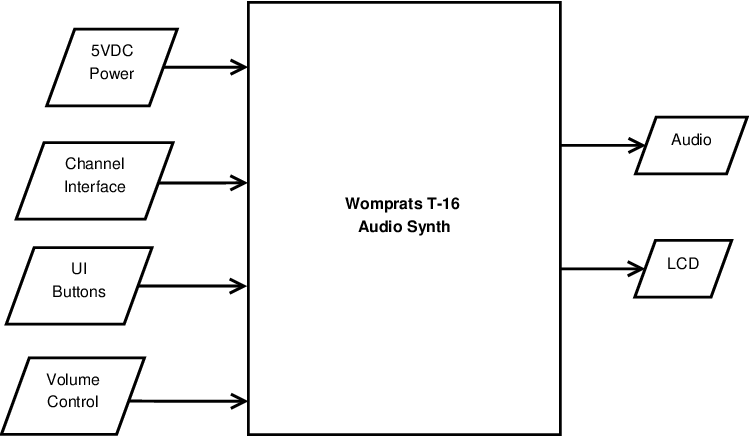
\includegraphics[width=5in]{synth0.png}}{Level 0 Diagram}{fullzero}

\begin{tabular}{|p{1in}|p{5in}|}
\hline
\emph{Module} & T-16 Audio Synthesizer \\
\hline
\emph{Inputs}& Lorem Ipsum\\
\hline
\emph{Outputs}& Dolor Sic \\ 
\hline
\emph{Functionality}& Bacon\\
\hline
\end{tabular}

\section{T-16 Audio Synthesizer Level 1 Diagram}
\centerimage{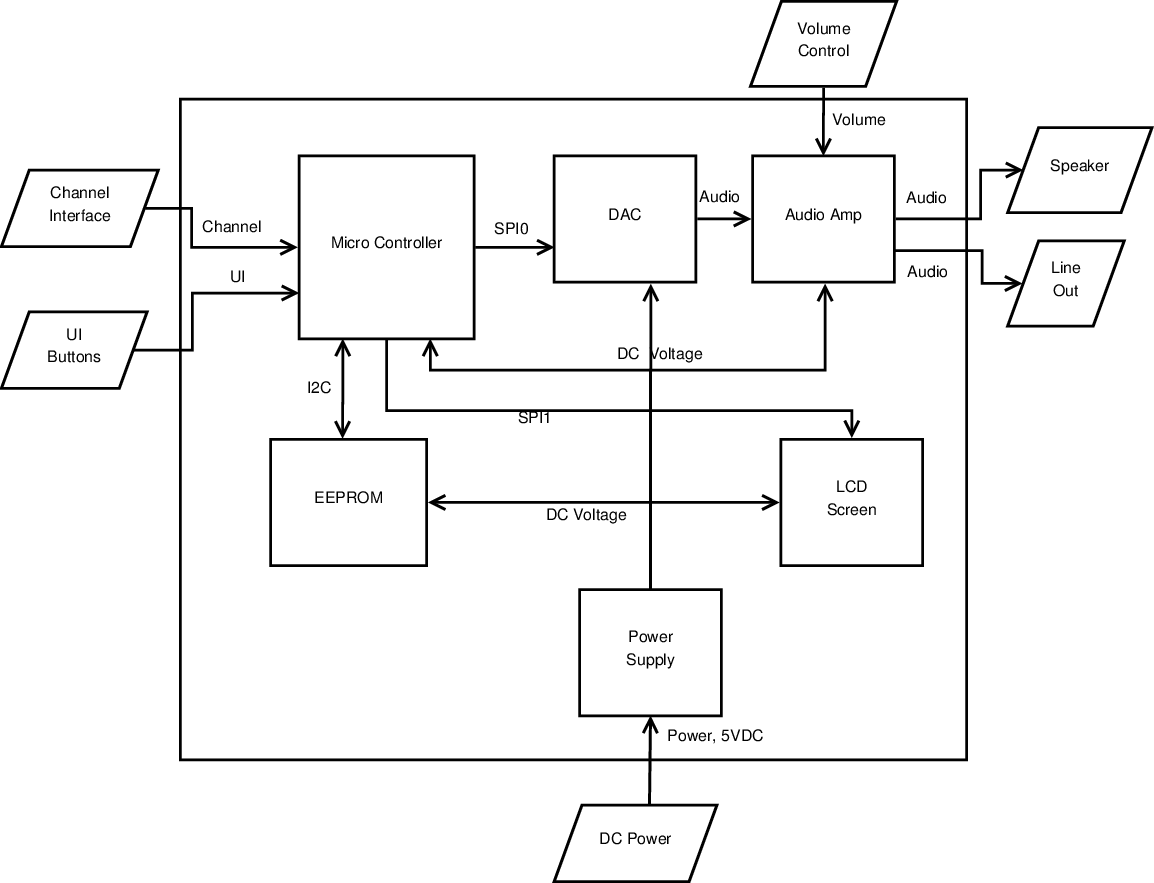
\includegraphics[width=5in]{synth1.png}}{Level 1 Diagram}{fullone}


\section{LCD Level 0 Diagram}
\centerimage{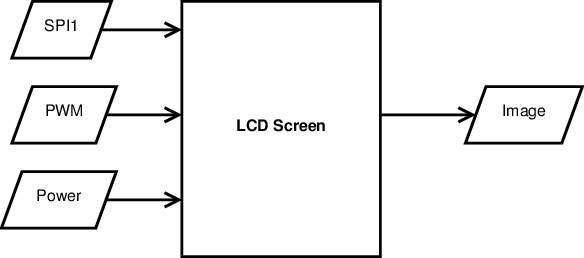
\includegraphics[width=5in]{lcd.png}}{Level 0 Diagram}{LCD}

\begin{tabular}{|p{1in}|p{5in}|}
\hline
\emph{Module} & LCD \\
\hline
\emph{Inputs}& Lorem Ipsum\\
\hline
\emph{Outputs}& Dolor Sic \\ 
\hline
\emph{Functionality}& Bacon\\
\hline
\end{tabular}

\section{Power Supply Level 0 Diagram}
\centerimage{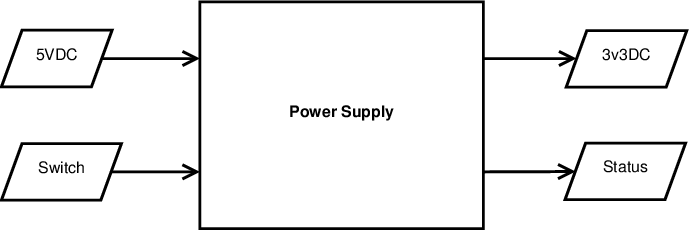
\includegraphics[width=5in]{pwrsply.png}}{Level 0 Diagram}{PSU}

\begin{tabular}{|p{1in}|p{5in}|}
\hline
\emph{Module} & Power Supply \\
\hline
\emph{Inputs}& Lorem Ipsum\\
\hline
\emph{Outputs}& Dolor Sic \\ 
\hline
\emph{Functionality}& Bacon\\
\hline
\end{tabular}

\section{EEPROM Level 0 Diagram}
\centerimage{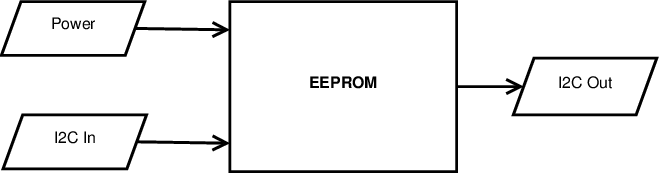
\includegraphics[width=5in]{eeprom.png}}{Level 0 Diagram}{eeprom}

\begin{tabular}{|p{1in}|p{5in}|}
\hline
\emph{Module} & EEPROM \\
\hline
\emph{Inputs}& Lorem Ipsum\\
\hline
\emph{Outputs}& Dolor Sic \\ 
\hline
\emph{Functionality}& Bacon\\
\hline
\end{tabular}

\section{Microcontroller Level 0 Diagram}
\centerimage{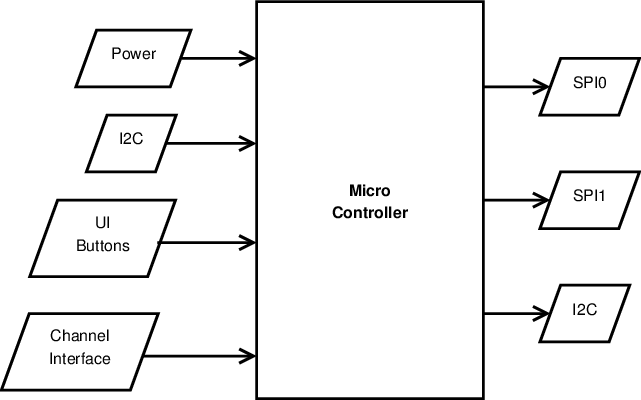
\includegraphics[width=5in]{microcont.png}}{Level 0 Diagram}{micro}

\begin{tabular}{|p{1in}|p{5in}|}
\hline
\emph{Module} & Microcontroller \\
\hline
\emph{Inputs}& Lorem Ipsum\\
\hline
\emph{Outputs}& Dolor Sic \\ 
\hline
\emph{Functionality}& Bacon\\
\hline
\end{tabular}

\section{DAC Level 0 Diagram}
\centerimage{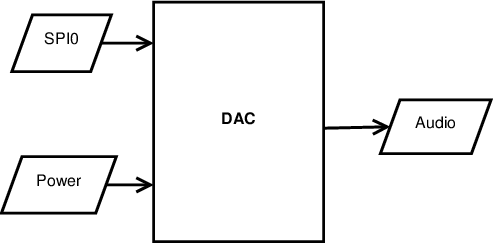
\includegraphics[width=5in]{dac.png}}{Level 0 Diagram}{dac}

\begin{tabular}{|p{1in}|p{5in}|}
\hline
\emph{Module} & DAC \\
\hline
\emph{Inputs}& Lorem Ipsum\\
\hline
\emph{Outputs}& Dolor Sic \\ 
\hline
\emph{Functionality}& Bacon\\
\hline
\end{tabular}

\section{Audio Amplifier Level 0 Diagram}
\centerimage{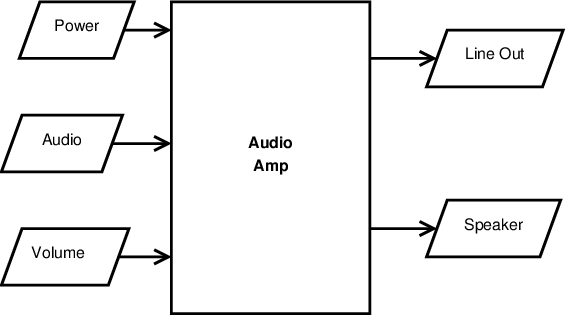
\includegraphics[width=5in]{audioamp.png}}{Level 0 Diagram}{audio}

\begin{tabular}{|p{1in}|p{5in}|}
\hline
\emph{Module} & Audio Amplifier \\
\hline
\emph{Inputs}& Lorem Ipsum\\
\hline
\emph{Outputs}& Dolor Sic \\ 
\hline
\emph{Functionality}& Bacon\\
\hline
\end{tabular}



\end{document}
